% data_ex.tex
\documentclass[main.tex]{subfiles}
\begin{document}
\chapter{Data Exploration} \label{ch:data_ex}
\section{Foreword} \label{sec:fw_dataex}

Material Extrusion (ME), also known as Fused Filament Fabrication (FFF), is the most prevalent Additive Manufacturing (AM) technology due to the broad range of materials and equipment available, generally attainable at a fraction of the cost of other AM processes. While ME has gradually found niche applications outside of the casual user, including implementations in the automotive and aerospace sectors, the slow print speed of the process represents a major pain point of the technology that limits the scope of its adoption. Additionally, process control relies mostly on temperature readings, and there is room for improvement in terms of variations in volumetric throughput and process fluctuations. For this reason, this study uses a customized ME machine with a built-in force sensor and encoder that allows real time acquisition of force and filament print speed data, generating knowledge aimed at maximizing the print speed of ME and improving the understanding of the underlying process physics that can lead to improved print quality and consistency. 

In the context of this dissertation, every ML solution begins with a data acquisition and exploration step. This study represents just that, as it allowed the researcher to understand an FFF machine with sensors, develop data filtering techniques, and the deployment of automation protocols that made acquisition of the training and validation data sets of the ML model a lot easier and faster. Finally, and as an added bonus, the results of this study shed some light into the current limitations intrinsic to two of the most widely used melting models for FFF: the Bellini \emph{et al.} model, and the Osswald, Puentes, Kattinger model, as both require measurements of filament force and speed to compare data with theoretical predictions \textemdash a feat that was uncommon at the time of this body of work.

\section{Equipment and Materials} \label{ssec:mat_data}

\subsection{Printer Setup} \label{ssec:printer}

For this study, an ME 3D printer (Minilab by FusedForm, Colombia) using a 0.4 mm nozzle and capable of printing 1.75 mm filament was equipped with a customized force sensor and thermistor built into the printhead, as well as an encoder that records the extruded filament length over time. The concentric force sensor was positioned just above the hot end, in a Bowden extruder architecture. These modifications permit recording and visualization of live force, filament speed, and temperature data collected during the printing process, while maintaining the original performance and functionality of the 3D printer. The generated data was collected using an Arduino board sampling at a frequency of 5 Hz, connected to MATLAB for visualization, processing, and logging. The printhead setup and encoder positioning can be seen in detail in Figure \ref{fig:printsetup}. This setup has the added benefit of allowing detection of filament slippage, if present. As shown in Figure \ref{fig:printsetup} the external ring of the force sensor sits on the extruder carrier base, secured by the extruder carrier lid. The modified hot-end sits on the internal ring of the force sensor, secured in place by the hot-end-sensor coupler. A small clearance between the carrier lid and the sensor permits the filament force to be transmitted through the assembly and detected by the DAQ system.

\begin{figure}[!htbp]
	\center
	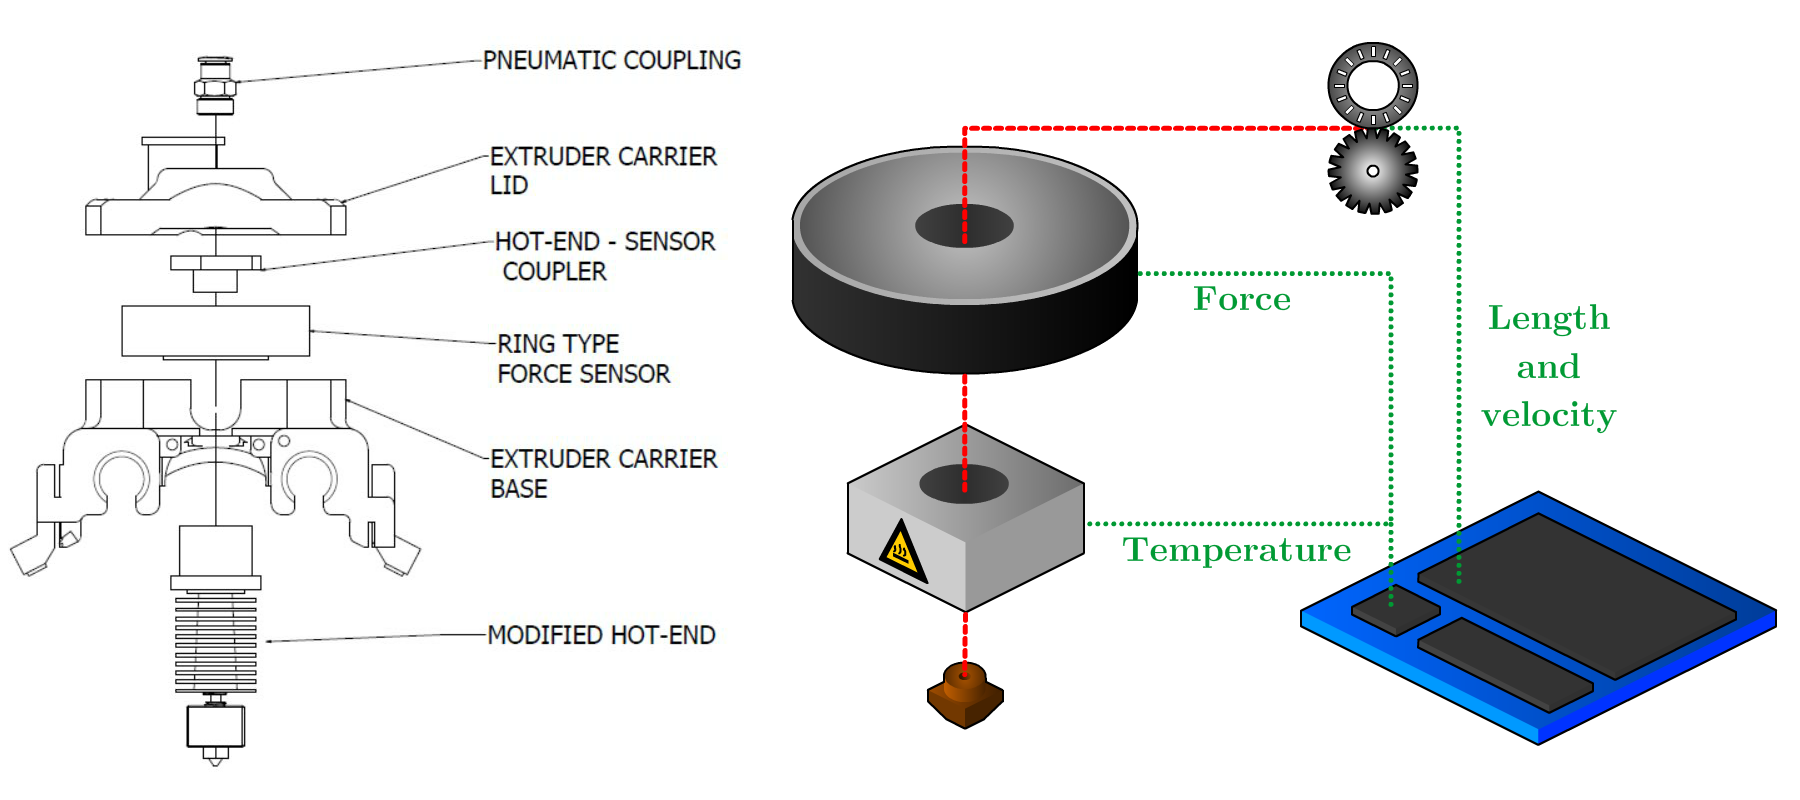
\includegraphics[width=0.9\linewidth, keepaspectratio]{Forcesetup}
	\caption{Assembly shown on the left. Schematic of sensor placement on the right.} \label{fig:printsetup}
\end{figure}

\subsection{Materials} \label{ssec:materials_dataex}

Two materials were chosen to perform the experiments pertaining to this body of work: a customized ABS filament, extruded in-house, and a commercially available PLA filament, each with a nominal diameter of 1.75 mm. The ABS filament was produced using the SABIC Cycolac™ MG94 material. This is an ABS resin traditionally used for injection molding thin-walled parts, as well as ME filament. With a reported Melt Flow Index of 11.7 g/10 min, it is an ideal resin for both the ME and extrusion processes \cite{sabic2016}. The extrusion setup consisted of a single screw extruder (Extrudex EDN 45X30D, Germany) with 45 mm screw diameter and L/D ratio of 30D. The hot melt was extruded at 205 ºC through a circular die with a 4.2 mm diameter. It was then guided through a pre-skinner into a vacuum-assisted, heated water bath (Conair, USA) to cool the extrudate whilst minimizing void formation. The solidified filament then passes through a 3-axis laser micrometer (LaserLinc, USA) and a belt puller (Conair, USA) in a control loop that allows adjustment of the pull speed to keep the extrudate within specification. The desired filament dimensions were a diameter of 1.75 mm with a tolerance of ±0.02 mm. A schematic of the extrusion setup can be seen in Figure \ref{fig:ex_line}. The PLA filament used was the commercially available "Natural PLA PRO" filament sold by Matterhackers, chosen to minimize the effect of colorants/additives to the composition of the filament. Steps were taken to ensure that all the acquired spools of material came from the same lot as to guarantee that processing conditions during the extrusion process were constant. Figure \ref{fig:rheo} shows the complex viscosity for each material, as measured using a 25 mm parallel plate rheometer and a 1 mm gap \cite{ColonQuintana2020}.

\begin{figure}[!htbp]
	\center
	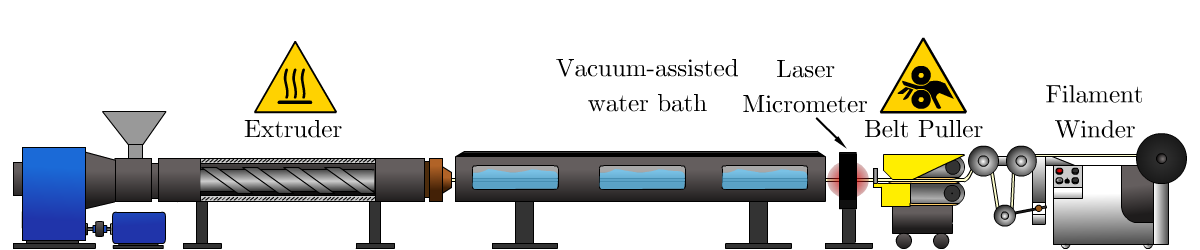
\includegraphics[width=0.9\linewidth, keepaspectratio]{Extrusion_line}
	\caption{Extrusion line used to produce ABS filament} \label{fig:ex_line}
\end{figure}

\begin{figure}[!htbp]
	\center
	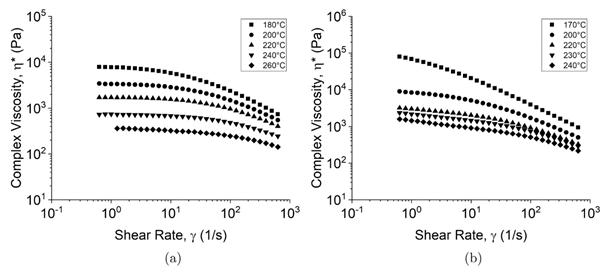
\includegraphics[width=\linewidth, keepaspectratio]{rheology}
	\caption{Shear rate dependency for a) PLA and b) ABS} \label{fig:rheo}
\end{figure}

\section{Design of Experiments} \label{sec:doe_data_ex}

A set of preliminary prints were designed with the goal of exploring the raw data, post processing requirements, and detection of lurking variables. In these experiments, the effect of temperature and print speed upon stable printing conditions in terms of required filament force was observed through the execution of several cylindrical toolpath files, where the printhead movement velocity was changed from 15 mm/s in increments of 5 mm/s every 15 layers, each with a thickness of 0.35 mm. To minimize the effects of varying accelerations during the test, a cylindrical geometry with a radius of 75 mm, printed in continuous helical mode was chosen as the benchmark part, as schematized in Figure \ref{fig:cyl_shak}. This ensures that changes in filament force and velocity stem mostly from the extrusion process and not due to toolpath considerations. To verify the effect of print temperature upon the required extrusion force, each material was printed at three different temperatures: 200, 215 and 230°C for PLA, and 215, 230 and 245°C for ABS. Close attention was paid to variability between prints performed at the same print conditions, as well as the maximum stable print speed for each material-temperature pairing.

\begin{figure}[!htbp]
	\center
	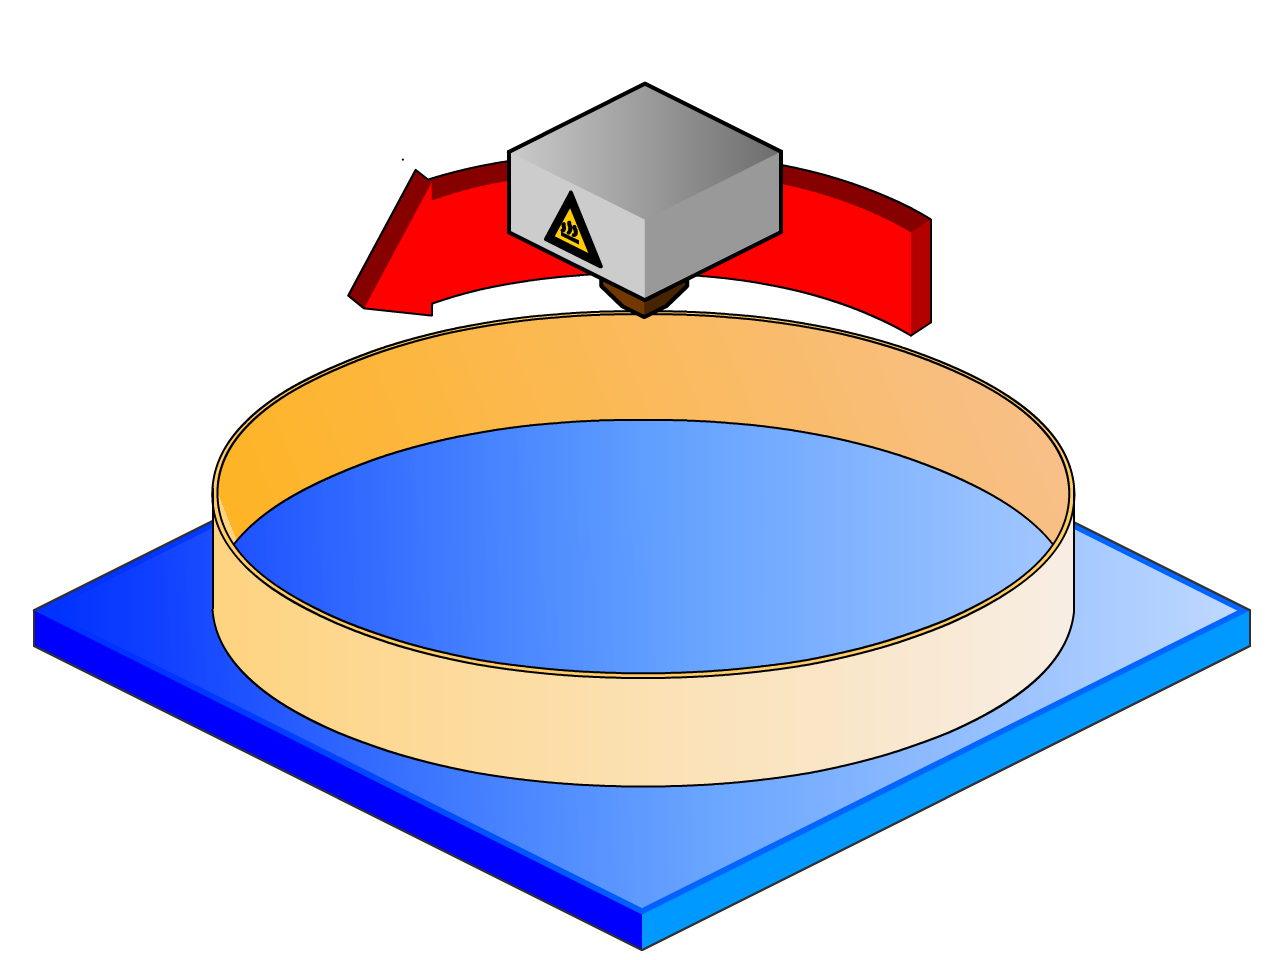
\includegraphics[width=0.6\linewidth, keepaspectratio]{cyl_shakira}
	\caption{Helical cylinder experiment} \label{fig:cyl_shak}
\end{figure}

Once conclusions were drawn from the preliminary set of experiments, the same geometry would be reprinted using a toolpath file that guarantees a comparable number of data points to be collected for each print speed-print temperature-material pairing, as well as utilizing optimal printing conditions and data acquisition considerations. 

\section{Results}
\subsection{Considerations Derived from Preliminary Tests}

Preliminary tests show that the physical limitation of the setup lies between 20 and 25 N of force acting upon the filament. At this level of force, slippage occurs in the drive wheel mechanism that drives the material towards the nozzle, causing the mass throughput to become discontinuous. This behavior manifested itself on the data as a sudden drop in the measured filament force and was accompanied by an audible click on the driving wheel. Each material-temperature pairing reached this threshold at different print speeds. Once this phenomenon was observed in a recurring manner, data acquisition was stopped to minimize the number of outliers and noise.
 
The characteristics of the ME printing process can be best described using a 2D plot, calculating the filament speed against the force within the nozzle. Filament speed is derived from the length data of extruded filament recorded by an encoder, and should not be confused with the printhead movement speed, which is followed by the machine after interpreting gcode.
 
Figure \ref{fig:unp_data} shows the unprocessed signals of length (bottom), the derived speed (middle) and resulting force (top) of a representative test print, made using PLA printed at 230°C. When looking at the plots of unprocessed signals, noise can be observed in the datasets of force and filament speed. Therefore, a combination of visualization and simple signal processing techniques are required to improve the signal to noise ratio of the datasets.

\begin{figure}[!htbp]
	\center
	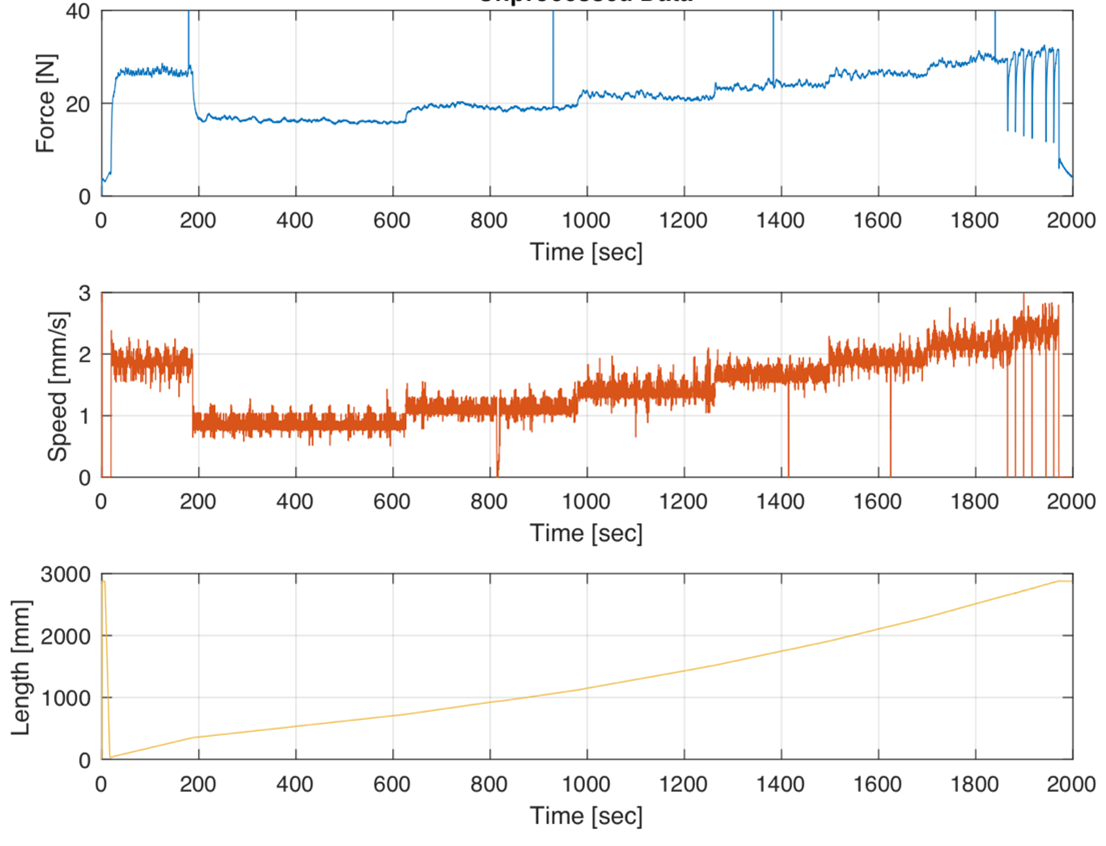
\includegraphics[width=\linewidth, keepaspectratio]{unp_signal}
	\caption{Raw signal data length (bottom), derived speed (middle), and force (top).} \label{fig:unp_data}
\end{figure}

In this example, the first 200 seconds of data are eliminated, as these constitute the time necessary to add the brim to the print, which is necessary to stabilize the cylinder. Datapoints above 1800 seconds are removed as well due to slippage of the filament and high variability within the signal. To remove the amplified noise of the derived speed signal, a moving average filter, applied to the length data showed the best results while keeping most of the signal information. Different parameters for the sliding window of length $k$ across neighboring elements of the length signal have been tested and number of 20 has been found most effective for this application, using a total of 7100 points in the dataset. Deriving the processed length data using the moving average with a sliding window $k$ of 20 shows good results on the filament speed signal in comparison with the unprocessed speed signal.  

% Nomenclature introduced in this chapter:
\nomenclature[A]{ME}{Material Extrusion}% 

\end{document}